\documentclass[12pt]{article}
 \usepackage[margin=1in]{geometry} 
\usepackage{amsmath,amsthm,amssymb,amsfonts}
 \usepackage{xcolor}
\newcommand{\N}{\mathbb{N}}
\newcommand{\Z}{\mathbb{Z}}
 \usepackage{graphicx,latexsym,amssymb}
 \usepackage{subcaption}
 \usepackage{parskip}
 \usepackage{epsfig}
 \usepackage{listings}
\usepackage{xcolor}
\usepackage{algpseudocode}
\usepackage{algorithm}
\usepackage{listings}
\usepackage{xcolor}
\usepackage{breqn}
\usepackage[english]{babel}
\usepackage{amsthm}
\newcommand\norm[1]{\left\lVert#1\right\rVert}
\newcommand\normx[1]{\left\Vert#1\right\Vert}
\usepackage{amssymb}
\usepackage{booktabs}
\newtheorem{theorem}{Theorem}[section]
\newtheorem{claim}[theorem]{Claim}
%\usepackage{mcode}
% Syntax: \colorboxed[<color model>]{<color specification>}{<math formula>}
\newcommand*{\colorboxed}{}
\def\colorboxed#1#{%
  \colorboxedAux{#1}%
}
\newcommand*{\colorboxedAux}[3]{%
  % #1: optional argument for color model
  % #2: color specification
  % #3: formula
  \begingroup
    \colorlet{cb@saved}{.}%
    \color#1{#2}%
    \boxed{%
      \color{cb@saved}%
      #3%
    }%
  \endgroup
}
\usepackage{epsfig}
\newenvironment{problem}[2][Problem]{\begin{trivlist}
\item[\hskip \labelsep {\bfseries #1}\hskip \labelsep {\bfseries #2.}]}{\end{trivlist}}
\lstset { %
    language=C++,
    backgroundcolor=\color{black!5}, % set backgroundcolor
    basicstyle=\footnotesize,% basic font setting
}
%If you want to title your bold things something different just make another thing exactly like this but replace "problem" with the name of the thing you want, like theorem or lemma or whatever
\algdef{SE}% flags used internally to indicate we're defining a new block statement
[STRUCT]% new block type, not to be confused with loops or if-statements
{Struct}% "\Struct{name}" will indicate the start of the struct declaration
{EndStruct}% "\EndStruct" ends the block indent
[1]% There is one argument, which is the name of the data structure
{\textbf{struct} \textsc{#1}}% typesetting of the start of a struct
{\textbf{end struct}}% typesetting the end of the struct
\begin{document}
\title{Project 1: Finite Difference Methods}
\author{Gaurav Dhir}
\maketitle
\section{Solution 1}
\subsection{Part (a)}
The order of the truncation error can be calculated by putting the exact solution within the discretization and by analyzing the remainder term obtained after Taylor Series expansions of the constituent terms around the point $x = x_j$. The exact differential equation has been stated in Equation \ref{eqdiff}.
\begin{equation} \label{eqdiff}
    \begin{aligned}
       & \frac{d  }{dx} \left( \kappa(x) \frac{d u(x)}{dx} \right) = f(x)  \\
       & or \quad \kappa'(x)\frac{d u(x)}{dx}+ \kappa(x) \frac{d^2 u(x)}{dx^2} = f(x)
    \end{aligned}
\end{equation}
The second order accurate discretization of Equation \ref{eqdiff} has been stated in Equation \ref{eqdis}. Here, $T(x_j)$ has been considered to be the truncation error of the discretization. 
\begin{equation} \label{eqdis}
    \begin{aligned}
       & \widetilde{D_0}u(x_j) = \frac{u(x_j + h/2) - u(x_j - h/2)}{h} \\
       & \widetilde{D_0}\left(\kappa(x_j)\widetilde{D_0}u(x_j) \right) = f(x_j) + T(x_j)
    \end{aligned}
\end{equation}
We can further expand the discretization scheme as shown in Equation \ref{eqexpand}.
\begin{equation} \label{eqexpand}
    \begin{aligned}
        & \frac{( \kappa(x) \widetilde{D_0} u(x) )_{x = x_j + h/2} - ( \kappa(x) \widetilde{D_0} u(x) )_{x = x_j - h/2}}{h} = f(x_j) + T(x_j) \\
        & \frac{\kappa(x_j + h/2) \left( u(x_j + h) - u(x_j) \right) - \kappa(x_j - h/2) \left( u(x_j) - u(x_j - h) \right)}{h^2} = f(x_j) + T(x_j)    
    \end{aligned}
\end{equation}
The final expanded discretization is shown in Equation \ref{eqfinal}.
\begin{equation} \label{eqfinal}
    \begin{aligned}
        &\frac{\kappa(x_j + h/2)u(x_j + h) - u(x_j)\left(\kappa(x_j + h/2) + \kappa(x_j - h/2)\right) + \kappa(x_j - h/2)u(x_j - h)}{h^2} -f(x_j) \\
        &  \quad \quad \quad \quad \quad \quad \quad \quad \quad \quad \quad \quad \quad \quad \quad \quad \quad \quad \quad \quad = T(x_j)
    \end{aligned}
\end{equation}
Since, $\kappa(x)$ and $u(x)$ are smooth functions of $x$, it is possible to perform a Taylor series expansion of these functions around the point $x_j$. The Taylor series expansions have been described in Equation \ref{eqtaylor}.
\begin{equation}\label{eqtaylor}
    \begin{aligned}
        & \kappa(x_j + h/2) = \kappa(x_j) + \frac{h}{2}\kappa'(x_j) + \frac{h^2}{8} \kappa''(x_j) + \frac{h^3}{48} \kappa'''(x_j) + \frac{h^4}{24 \times 16} \kappa''''(x_j) + O(h^5) \\
        & \kappa(x_j - h/2) = \kappa(x_j) - \frac{h}{2}\kappa'(x_j) + \frac{h^2}{8} \kappa''(x_j) - \frac{h^3}{48} \kappa'''(x_j) + \frac{h^4}{24 \times 16} \kappa''''(x_j) + O(h^5) \\
        & u(x_j + h) =  u(x_j) + h u'(x_j) + \frac{h^2}{2} u''(x_j) + \frac{h^3}{6} u'''(x_j) + \frac{h^4}{24} u''''(x_j) + O(h^5) \\
        & u(x_j - h) =  u(x_j) - h u'(x_j) + \frac{h^2}{2} u''(x_j) - \frac{h^3}{6} u'''(x_j) + \frac{h^4}{24} u''''(x_j) + O(h^5) \\
    \end{aligned}
\end{equation}
Using the Taylor expansions of the relevant terms shown in Equation \ref{eqtaylor}, it is now possible to calculate the truncation error $T(x_j)$ shown in Equation \ref{eqfinal}. The expression for $T(x_j)$ is shown in Equation \ref{eqtrunc}.
\begin{equation} \label{eqtrunc}
    \begin{aligned}
        & T(x_j) = \kappa'(x_j)u'(x_j)+ \kappa(x_j) u''(x_j) - f(x_j) + \\
        & h^2 \left( \frac{\kappa(x_j) u''''(x_j)}{12} + \frac{\kappa'(x_j) u'''(x_j)}{6} + \frac{\kappa''(x_j) u''(x_j)}{8} + \frac{\kappa'''(x_j) u'(x_j)}{24}  \right) + O(h^3)
    \end{aligned}
\end{equation}
We know from Equation \ref{eqdiff} that the exact differential equation satisfies $ \kappa'(x_j)u'(x_j)+ \kappa(x_j) u''(x_j) - f(x_j) = 0$. Hence, the final expression for the truncation error of the expansion is shown in Equation \ref{finaltrunc}.
\begin{equation}\label{finaltrunc}
    T(x_j) = h^2 \left( \frac{\kappa(x_j) u''''(x_j)}{12} + \frac{\kappa'(x_j) u'''(x_j)}{6} + \frac{\kappa''(x_j) u''(x_j)}{8} + \frac{\kappa'''(x_j) u'(x_j)}{24} \right) + O(h^3) 
\end{equation}
We find that the final expression for the Truncation error as displayed in Equation \ref{finaltrunc} has a term which is $O(h^2)$. Hence, we can conclude that the discretization has second order local truncation error.
\subsection{Part (b)}
Using the method of manufactured solutions, an exact solution was posited as shown in Equation \ref{eqexact}. It is easily observed that the exact solution satisfies the boundary conditions since at $x_j = 0$ and $x_j = 1$, the value of $sin(\pi x_j)$ is equal to $0$.
\begin{equation} \label{eqexact}
    u(x_j) = sin(\pi x_j)
\end{equation}
Also, $u'(x) = \pi cos(\pi x)$ and $ \kappa(x)u'(x) = 2 \pi cos(\pi x) + \pi cos(\pi x) \sum_{l = 1}^{l = 5} sin(l \pi x)/(l + 1) $. Using these expressions, the value of $f(x_j)$ was calculated and was found to be equal to the expression described in Equation \ref{eqf}
\begin{equation} \label{eqf}
\begin{aligned}
    & f(x) = \frac{d}{dx} \kappa(x) \frac{d}{dx} u(x) \\
    & or \quad f(x) = -2\pi^2 sin(\pi x) - \pi^2 sin(\pi x) \left( \sum_{l = 1}^{l = 5} \frac{sin(l \pi x)}{l + 1} \right) + l \pi^2 cos(\pi x) \left( \sum_{l = 1}^{l = 5} \frac{cos(l \pi x)}{ l + 1 } \right)
\end{aligned}
\end{equation}
\subsection{Part (c)}
The Partial Differential Equation was discretized and the Gauss Siedel Scheme was used to obtain the solution at different values of grid spacing. The discretized system of equations has been summarized in Equation \ref{eqdis}. Here $r$ denotes the iteration level of the scheme.
\begin{equation} \label{eqdis}
    \begin{aligned}
        & \frac{\kappa( x_j + h/2 ) u(x_j + h) + \kappa( x_j - h/2 )u( x_j - h ) - u(x_j)( \kappa(x_j + h/2) + \kappa(x_j - h/2) )}{h^2} = f(x_j) \\
        & where \quad j = 1, 2, \ldots, N - 1 \\
        & and \quad u(0) = 0, \quad u(1) = 0
    \end{aligned}
\end{equation}
\begin{equation} \label{eqdis}
    \begin{aligned}
        & u(x_j)^{r + 1} = \frac{h^2}{A} \left( \frac{ \left( \kappa(x_j + h/2)u(x_j + h)^{r} + \kappa(x_j - h/2) u(x_j - h)^{r + 1} \right)}{h^2} - f(x_j) \right) \\
        & where \quad A = \kappa(x_j + h) + \kappa(x_j - h)
    \end{aligned}
\end{equation}
The Gauss Siedel Iteration is continued until the $L^2$ norm of the residual converges below a tolerance value set to $1e-6$. A key component of grid convergence analysis is the mathematical framework used to calculate the error between the iterations. It is well known from Equation \ref{eqerror} that the error $e$ between the exact solution and the update at the current iteration is bounded by the residual $R$. Although the condition number also plays a key role but it is established that the error in the solution is bounded from above by the residual. A similar relationship was not found for the error given by $\norm{u^{r} - u^{r - 1}}_2$ where $u^r$ and $u^{r - 1}$ are the solution values at the current and the previous iterations respectively. As a result, the error between iterations was implemented in code using the residual. It must also be noted that a perfect convergence plot as shown in Figure \ref{errorplot} was not seen when the iteration error was calculated using the the error given by $\norm{u^{r} - u^{r - 1}}_2$.
\begin{equation}\label{eqerror}
    \frac{\norm{e}_2}{\norm{u}_2} \leq \norm{A}_2 \norm{A^{-1}}_2 \frac{\norm{R}_2}{\norm{f}_2}
\end{equation}
The Residual $R(x_j)$ was calculated using Equation \ref{res} and the scaled $L^2$ norm of the residual was used to evaluate the error.
\begin{equation} \label{res}
    \begin{aligned}
        & R(x_j) = \frac{\kappa( x_j + h/2 ) u(x_j + h) + \kappa( x_j - h/2 )u( x_j - h ) - u(x_j)( \kappa(x_j + h/2) + \kappa(x_j - h/2) )}{h^2} - f(x_j) \\
        & and \quad Error = \sqrt{ \frac{\sum_{j = 1}^{N - 1} R(x_j)^2}{N} }
    \end{aligned}
\end{equation}
Figure \ref{solplot} shows the plot of the solution $u(x_j)$ at $N = 65$ where $N$ represents the number of points on the grid used for discretization. Figure \ref{errorplot} shows the convergence plot of the error at different values of grid spacing. The slope of the error plot was calculated and was found to be equal to $2.06$ establishing perfect second order solution convergence. 
\begin{figure}
\centering
    {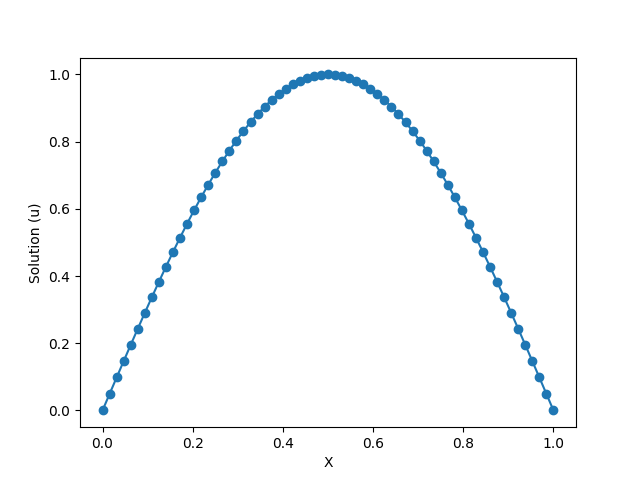
\includegraphics[width=14cm]{Solution_Plot_65.png} }%
    \caption{Solution Plot at $N = 65$}%
    \label{solplot}%
\end{figure}
\begin{figure}
\centering
    {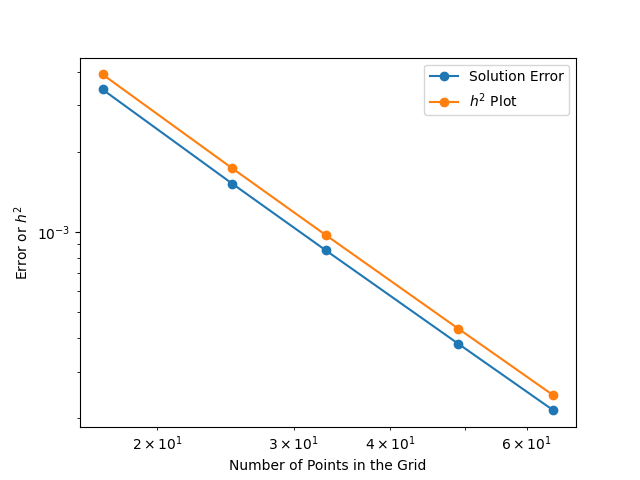
\includegraphics[width=14cm]{Error_Plot.png} }%
    \caption{Convergence Error Plot with Error calculation performed at various grid spacings}%
    \label{errorplot}
\end{figure}
\end{document}
